\section{RRTHull  Class Reference}
\label{classRRTHull}\index{RRTHull@{RRTHull}}
Grow a Rapidly-exploring Random Tree in a large disc. 


{\tt \#include $<$rrt.h$>$}

Inheritance diagram for RRTHull::\begin{figure}[H]
\begin{center}
\leavevmode
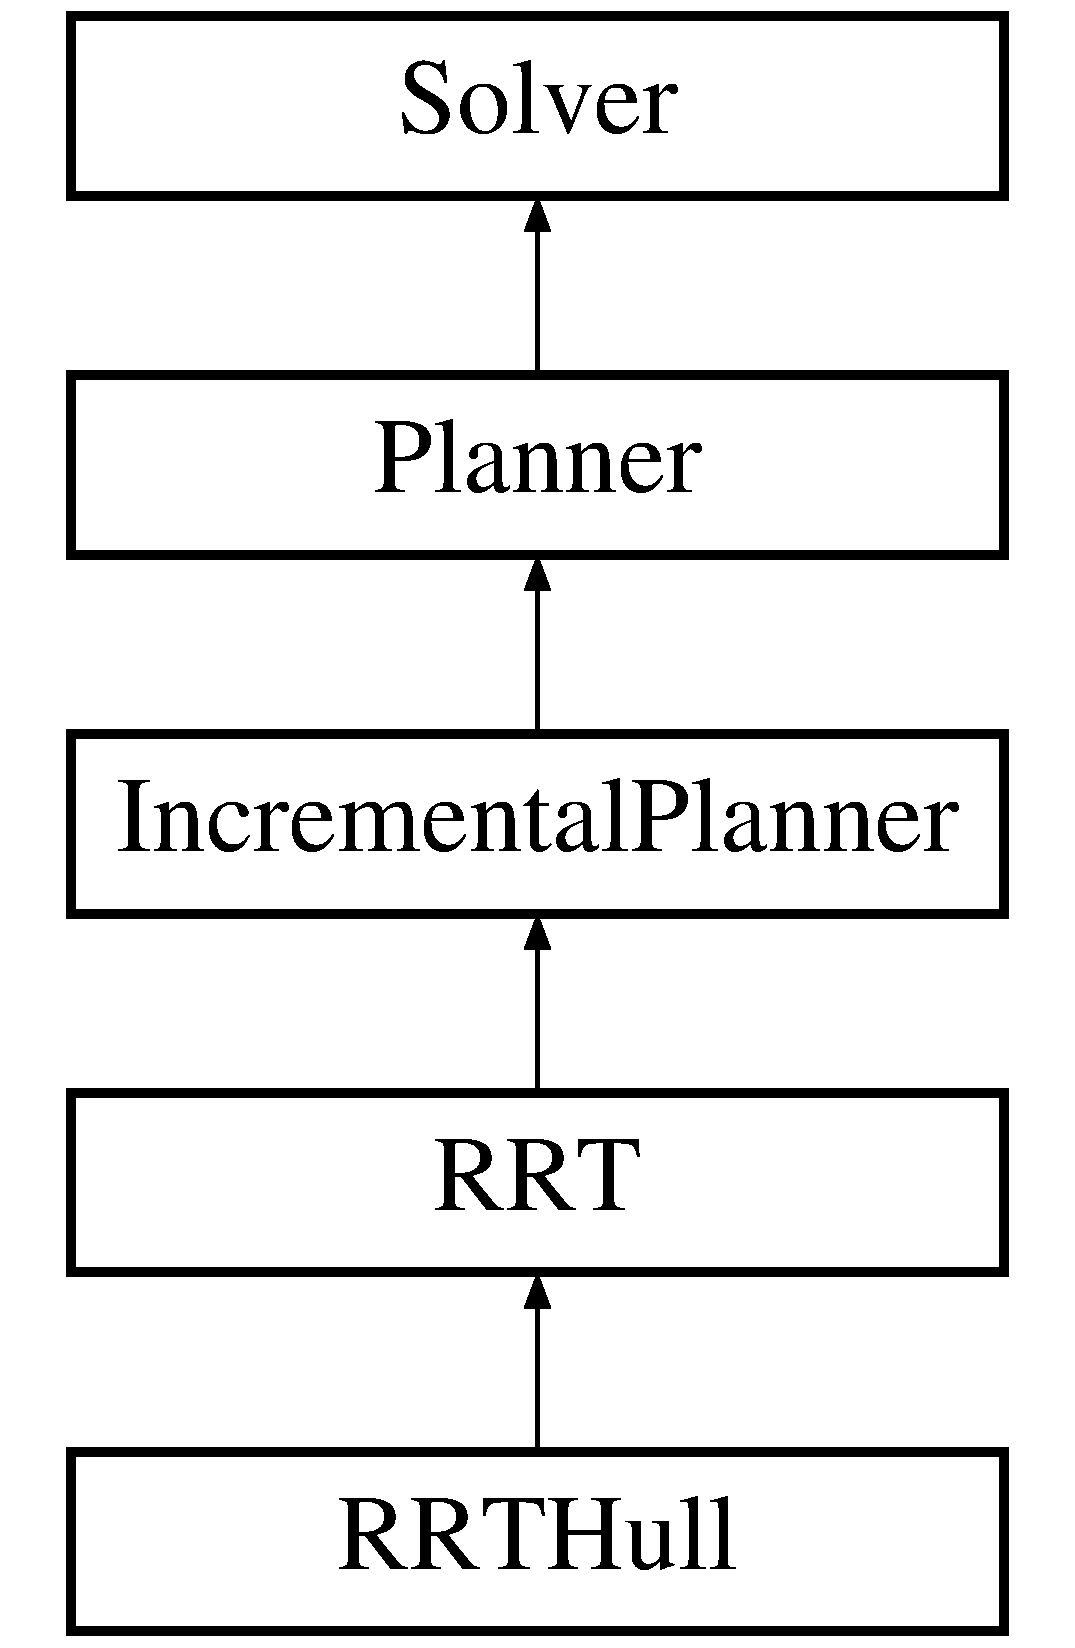
\includegraphics[height=5cm]{classRRTHull}
\end{center}
\end{figure}
\subsection*{Public Methods}
\begin{CompactItemize}
\item 
{\bf RRTHull} ({\bf Problem} $\ast$p)
\item 
virtual {\bf $\sim$RRTHull} ()
\end{CompactItemize}
\subsection*{Public Attributes}
\begin{CompactItemize}
\item 
double {\bf Radius}
\end{CompactItemize}
\subsection*{Protected Methods}
\begin{CompactItemize}
\item 
virtual {\bf MSLVector} {\bf Choose\-State} ()
\begin{CompactList}\small\item\em Pick a state using some sampling technique.\item\end{CompactList}\end{CompactItemize}


\subsection{Detailed Description}
Grow a Rapidly-exploring Random Tree in a large disc.

This is a special-purpose class that grows a tree in an \char`\"{}infinitely\char`\"{} large disc to study asymptotic properties. 



\subsection{Constructor \& Destructor Documentation}
\index{RRTHull@{RRTHull}!RRTHull@{RRTHull}}
\index{RRTHull@{RRTHull}!RRTHull@{RRTHull}}
\subsubsection{\setlength{\rightskip}{0pt plus 5cm}RRTHull::RRTHull ({\bf Problem} $\ast$ {\em p})}\label{classRRTHull_a0}


\index{RRTHull@{RRTHull}!~RRTHull@{$\sim$RRTHull}}
\index{~RRTHull@{$\sim$RRTHull}!RRTHull@{RRTHull}}
\subsubsection{\setlength{\rightskip}{0pt plus 5cm}virtual RRTHull::$\sim$RRTHull ()\hspace{0.3cm}{\tt  [inline, virtual]}}\label{classRRTHull_a1}




\subsection{Member Function Documentation}
\index{RRTHull@{RRTHull}!ChooseState@{ChooseState}}
\index{ChooseState@{ChooseState}!RRTHull@{RRTHull}}
\subsubsection{\setlength{\rightskip}{0pt plus 5cm}{\bf MSLVector} RRTHull::Choose\-State ()\hspace{0.3cm}{\tt  [protected, virtual]}}\label{classRRTHull_b0}


Pick a state using some sampling technique.



Reimplemented from {\bf RRT} {\rm (p.\,\pageref{classRRT_b4})}.

\subsection{Member Data Documentation}
\index{RRTHull@{RRTHull}!Radius@{Radius}}
\index{Radius@{Radius}!RRTHull@{RRTHull}}
\subsubsection{\setlength{\rightskip}{0pt plus 5cm}double RRTHull::Radius}\label{classRRTHull_m0}




The documentation for this class was generated from the following files:\begin{CompactItemize}
\item 
{\bf rrt.h}\item 
{\bf rrt.C}\end{CompactItemize}
